\iffalse
\let\negmedspace\undefined
\let\negthickspace\undefined
\documentclass[journal,12pt,twocolumn]{IEEEtran}
\usepackage{cite}
\usepackage{amsmath,amssymb,amsfonts,amsthm}
\usepackage{algorithmic}
\usepackage{graphicx}
\usepackage{textcomp}
\usepackage{xcolor}
\usepackage{txfonts}
\usepackage{listings}
\usepackage{enumitem}
\usepackage{mathtools}
\usepackage{gensymb}
\usepackage{comment}
\usepackage[breaklinks=true]{hyperref}
\usepackage{tkz-euclide} 
\usepackage{listings}
\usepackage{gvv}                                        
\def\inputGnumericTable{}                                 
\usepackage[latin1]{inputenc}                                
\usepackage{color}                                            
\usepackage{array}                                            
\usepackage{longtable}                              
\usepackage{calc}                                             
\usepackage{multirow}                                         
\usepackage{hhline}                                           
\usepackage{ifthen}                                           
\usepackage{lscape}

\newtheorem{theorem}{Theorem}[section]
\newtheorem{problem}{Problem}
\newtheorem{proposition}{Proposition}[section]
\newtheorem{lemma}{Lemma}[section]
\newtheorem{corollary}[theorem]{Corollary}
\newtheorem{example}{Example}[section]
\newtheorem{definition}[problem]{Definition}
\newcommand{\BEQA}{\begin{eqnarray}}
\newcommand{\EEQA}{\end{eqnarray}}
\newcommand{\define}{\stackrel{\triangle}{=}}
\theoremstyle{remark}
\newtheorem{rem}{Remark}
\begin{document}

\bibliographystyle{IEEEtran}
\vspace{3cm}

\title{GATE 2023 BM}
\author{EE23BTECH11020 - Raghava Ganji$^{*}$% <-this % stops a space
}
\maketitle
\newpage
\bigskip

\renewcommand{\thefigure}{\theenumi}
\renewcommand{\thetable}{\theenumi}

\textbf{GATE 2023 BM.48:}
The function $f(z)=\frac{1}{z-1}$ of a complex variable z on a closed contour in an anti-clockwise direction.For which of the following contours, does this integral have a non-zero value?\\
\brak{A}$\abs{z-2}=0.01$\\
\brak{B}$\abs{z-1}=0.1$\\
\brak{C}$\abs{z-3}=5$\\
\brak{D}$\abs{z}=2$\\
\solution\\
\fi
Cauchy's Integral Formula and Residue Theorem.
\begin{align}
\oint_{c}f\brak z&=2\pi jRes\sbrak{f\brak z,z_0}\label{eq:CIF}\\
Res\sbrak{f\brak z,z_0}&=\lim_{z\to z_0}\sbrak{\brak{z-z_0}f\brak z}\label{eq:Res Thm}
\end{align}
Here $z_0$ is pole of the f\brak z\\
Using \eqref{eq:CIF}
\begin{align}
\oint_{c}\frac{1}{z-1}dz &=2\pi jRes\sbrak{\frac{1}{z-1},1}
\end{align}
\begin{enumerate}
\item For option A the pole is outside the contour, then Residue is zero.\\
\begin{figure}[h!]
    \centering
    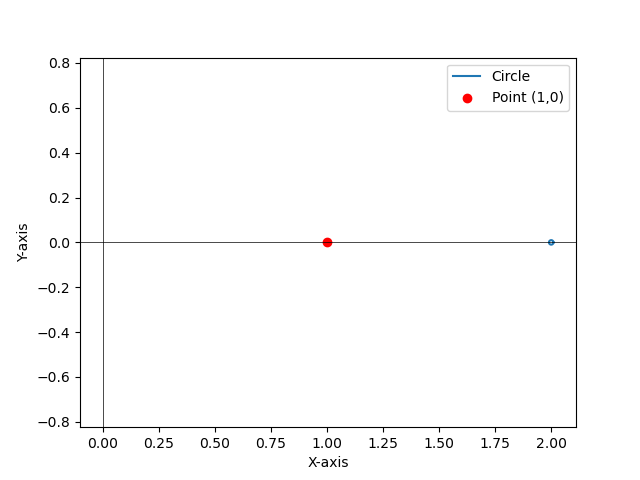
\includegraphics[width=1\columnwidth]{2023/BM/48/figs/plotg231.png}
    \caption{graph of option A}
\end{figure}
\begin{align}
\implies\oint_{c}\frac{1}{z-1}dz &=2\pi j\brak{0}\\
\implies 0
\end{align}
\item For option B the pole is inside the contour.\\
\begin{figure}[h!]
    \centering
    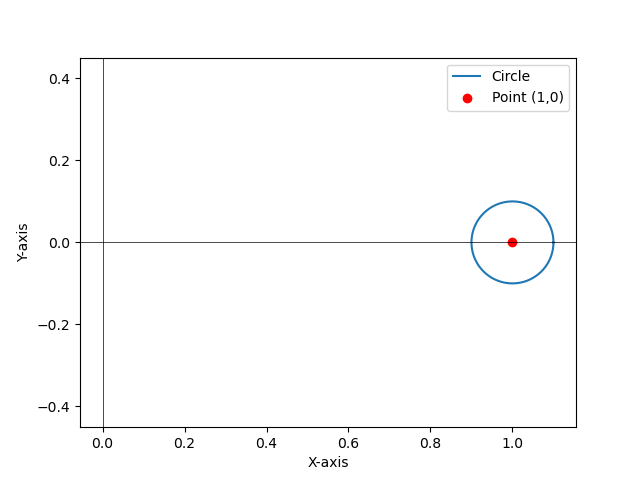
\includegraphics[width=1\columnwidth]{2023/BM/48/figs/plotg232.png}
    \caption{graph of option B}
\end{figure}
Then, using \eqref{eq:Res Thm}
\begin{align}
Res\sbrak{\frac{1}{z-1},1} &=\lim_{z\to 1}\brak{z-1}\frac{1}{z-1}\\
&=1\\
\implies \oint_{c}\frac{1}{z-1}dz&=2\pi j\brak 1\\
\implies 2\pi j
\end{align}
\item For option C the pole is inside the contour.\\
\begin{figure}[h!]
    \centering
    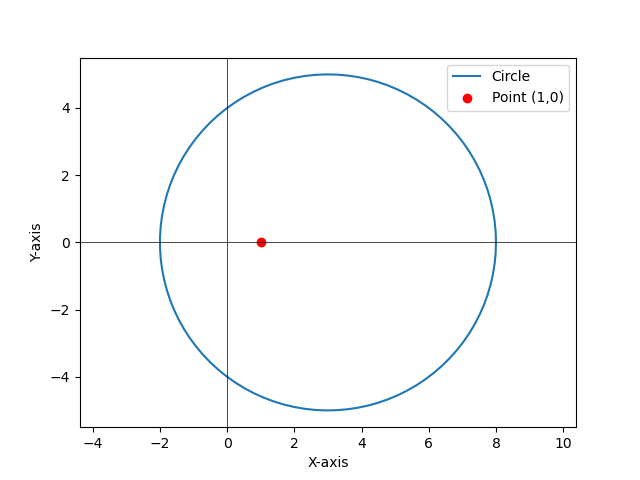
\includegraphics[width=1\columnwidth]{2023/BM/48/figs/plotg233.png}
    \caption{graph of option C}
\end{figure}
Then, using \eqref{eq:Res Thm}
\begin{align}
Res\sbrak{\frac{1}{z-1},1} &=\lim_{z\to 1}\brak{z-1}\frac{1}{z-1}\\
&=1\\
\implies \oint_{c}\frac{1}{z-1}dz&=2\pi j\brak 1\\
\implies 2\pi j
\end{align}
\item For option D the pole is inside the contour.\\
\begin{figure}[h!]
    \centering
    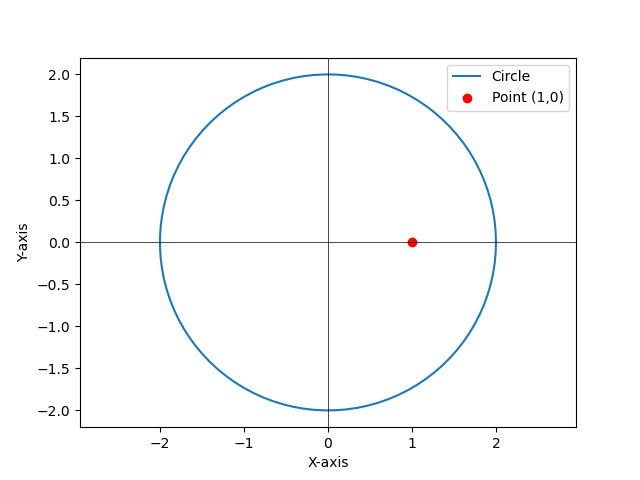
\includegraphics[width=1\columnwidth]{2023/BM/48/figs/plotg234.png}
    \caption{graph of option D}
\end{figure}
Then, using \eqref{eq:Res Thm}
\begin{align}
Res\sbrak{\frac{1}{z-1},1} &=\lim_{z\to 1}\brak{z-1}\frac{1}{z-1}\\
&=1\\
\implies \oint_{c}\frac{1}{z-1}dz&=2\pi j\brak 1\\
\implies 2\pi j
\end{align}
\end{enumerate}
We can conclude that for options B,C,D contours have the non-zero value for this integral.
%\end{document}
